\documentclass[a4paper]{article}
\usepackage[T1]{fontenc} % Polskie znaki
\usepackage{graphicx} % Wstwianie grafiki
\usepackage{subcaption}
%opening
\title{Rozpoznawanie stanu rozgrywki w grze planszowej Catan}
\author{Magdalena Wiechczyńska, \\
Piotr Tomaszewski, 136821}
\date{} %Usunięcie daty

\begin{document}

\maketitle

\section{Temat i opis rozwiązania problemu}

\section{Działanie programu}
    \subsection{Znajdowanie planszy}
    Na początku program próbuje ustalić położenie planszy i usunąć wszelkie elementy do niej nienależące.

    Wiedząc, że plansza do gry jest zawsze otoczona ramką przedstawiającą wodę, wyszukujemy pikseli, których wartość odcienia (Hue) w przestrzeni HSV należy do odpowiedniego przedziału. Następnie uzyskany obraz poddajemy dylatacji.
    \begin{figure}[h]
        \begin{subfigure}[]{.5\linewidth}
        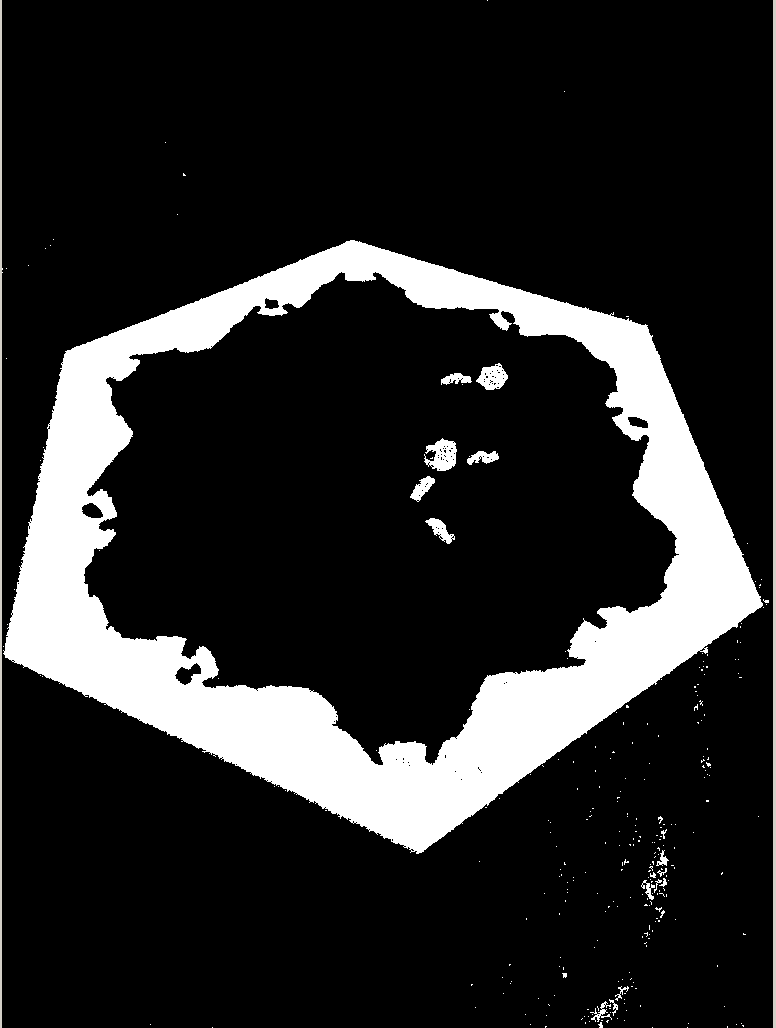
\includegraphics[width=\linewidth]{pictures/steps/find_water.png}
        \subcaption{Wycięta ramka}

        \end{subfigure}
        \begin{subfigure}[]{0.5\linewidth}
        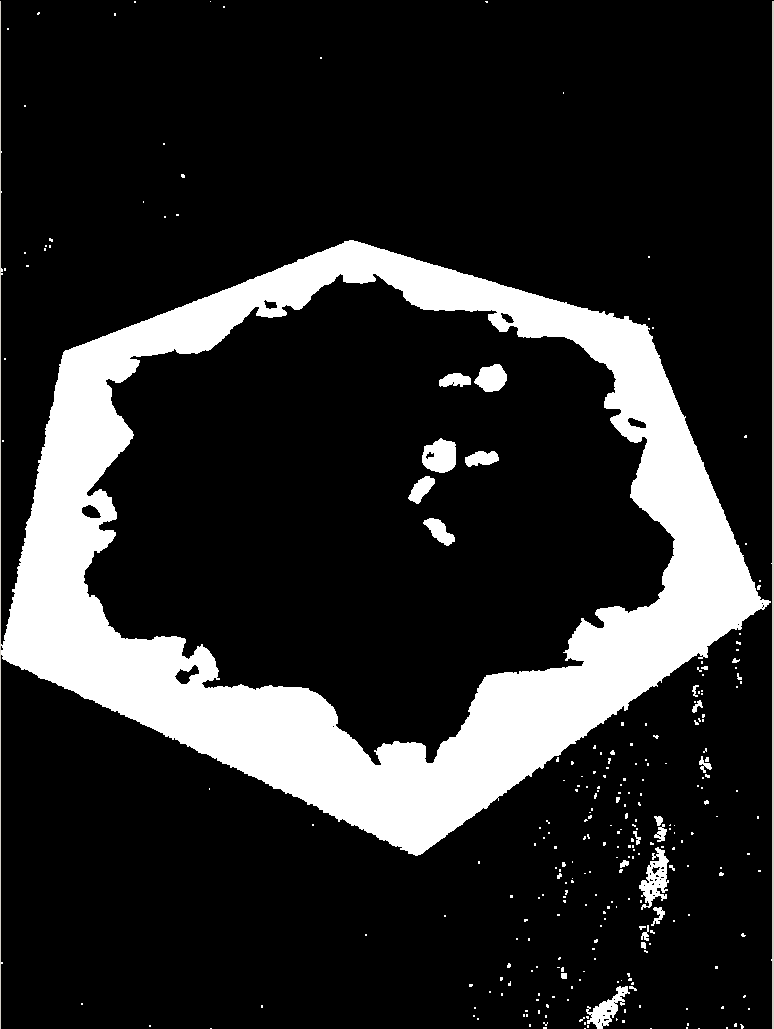
\includegraphics[width=\linewidth]{pictures/steps/find_water_dilate.png}
        \subcaption{Wycięta ramka poddana dylatacji}
        \end{subfigure}

        \caption{Znajdowanie ramki.}
        \label{fig:step1}
    \end{figure}

    Na tak przetworzonym obrazie szukamy konturów. Zależy nam na znalezieniu wewnętrznego konturu planszy. Na większości zdjęć jest to drugi kontur pod względem obejmowanego pola powierzchni. Jednak na niekórych fotografiach, zewnętrzny kontur łączy się z otoczeniem, przez co program go nie znajduje. Wówczas to wewnętrzny kontur staje się największy. W celu ustalenia, który kontur jest tym wewnętrznym, sprawdzamy czy drugi pod względem wielkości kontur znajduje się wewnątrz największego.

    \subsection{Znajdowanie pionków}

    \subsection{Rozpoznawanie pionków}

    \subsection{Znajdowanie i rozpoznawanie pól}
      
\section{Przedstawienie wyników}
    \subsection{Zdjęcia łatwe}
    \subsection{Zdjęcia średnie}
    \subsection{Zdjęcia trudne}
\section{Podsumowanie wyników}


\end{document}
